\chapter{Results}
In this chapter the proposed algorithm is evaluated on the LPW data set and numerical results are presented, followed by a discussion of the results and possible improvements.
\section{Evaluation}
The evaluation of the proposed algorithm is done by calculating the error of the pupil center. The data set has as label the center of the ellipse and but not the actual ellipse parameter. Therefore a evaluation of the actual fit of the ellipse was conducted manually and no numerical results for the fit are presented. For the evaluation of the pupil center, the ground truth notation explained in subsection \ref{subsec:ground_truth} is used. The error is calculated in x and y direction separately and a KDE Plot is used to display the error density of the estimation. The error is calculated of each frame, totaling 2000 frames per video. The standart deviation in calculated and draw into the KDE plos as an ellipse and gives insight into the acuraccy of the algorithm. The noise changes throughout the video because of eye movement and blinking. As already mentioned in the introduction, the algorithm is not able to detect if the eye is open or closed. Therefore a big deviation in the error is possible and is filtered out if it is bigger than three times the standart deviation of the complete video. To filter the error, the z score is introduced. The z score is a statistical measure that tells how far a point is from the mean of a data set in terms of standard deviations. For the evaluation all errors with a z score bigger than three are declared as outliers. 

\section{Discussion}
The performance of the algorithm can be split up into: Accuracy, Speed, Robustness and Noise. The accuracy is measured by the error of the pupil center. The speed is measured by the frames per second the algorithm can process. The robustness is measured by the amount of outliers the algorithm produces. The noise is hard to evaluate because the data set very diverse and there is eye movement during the video changing the amount of noise that is introduced.
\subsection{Accuracy}
The Accuracy of the algorithm can be seen in the KDE plot of an example video. The KDE plot is shown in figure \ref{fig:kde}. which shows the error density of the pupil center estimation. 

\begin{figure}[h]
        \centering
        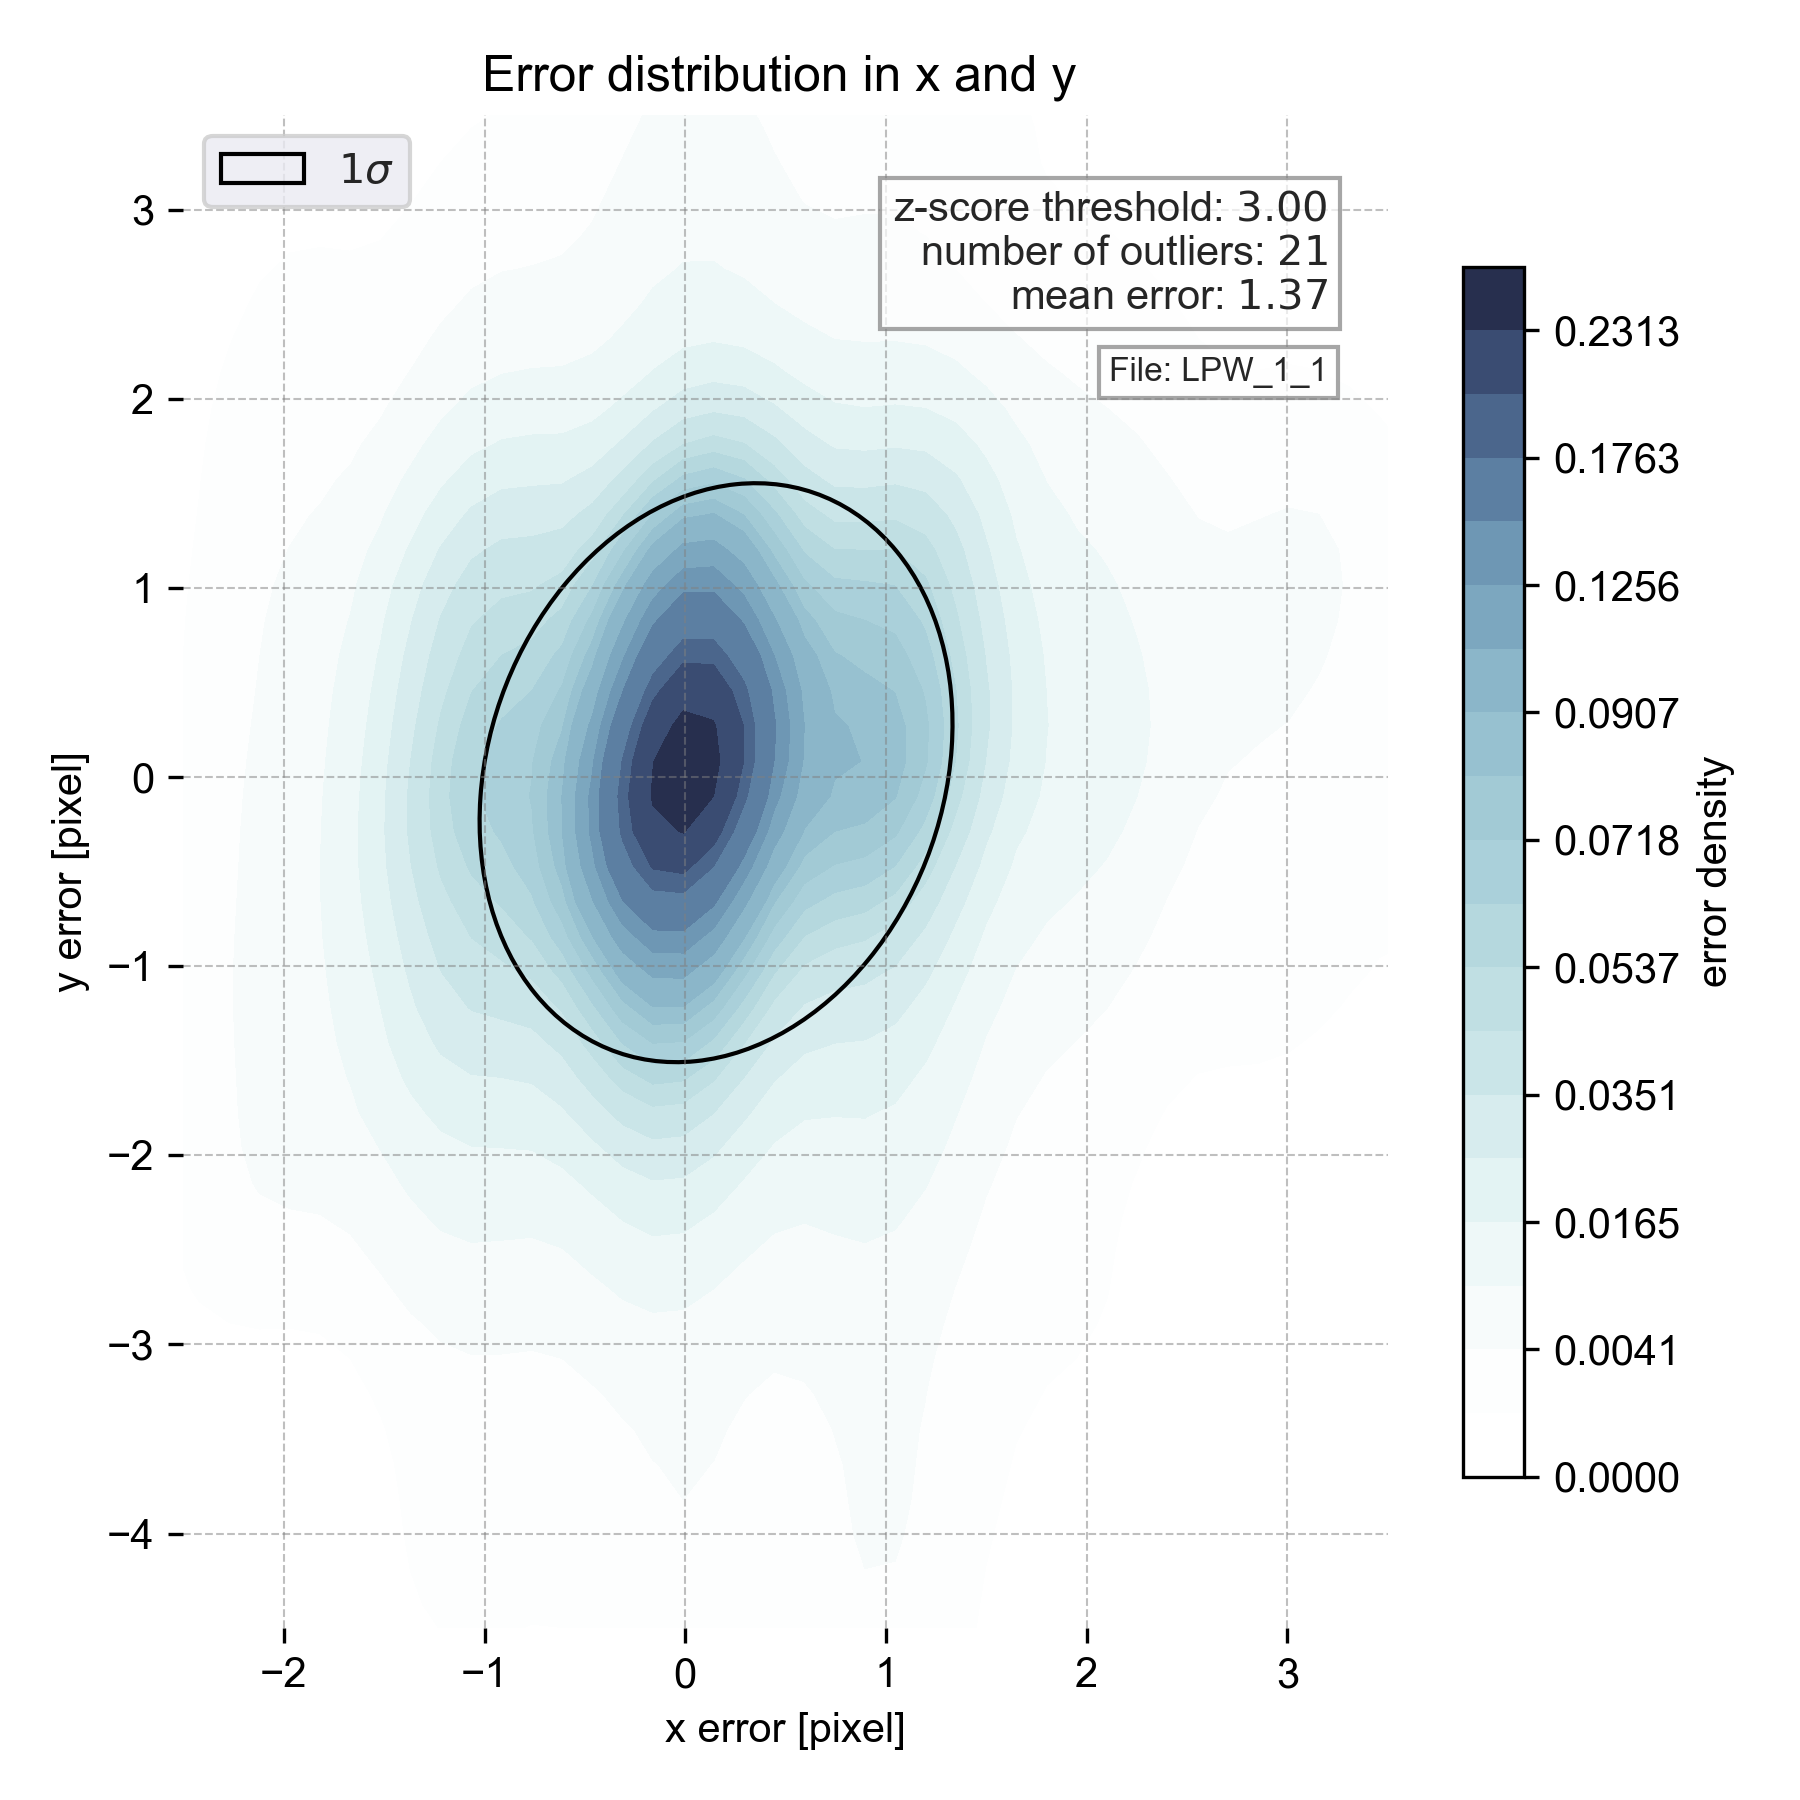
\includegraphics[width=\textwidth]{plots/LPW_1_1pre.png}
    \caption{Error KDE plot of the pupil center estimation}
    \label{fig:kde}
\end{figure}
Here it can be seen that the standard deviation in y direction is bigger than in x direction. This has to do with the experimental setup of the LPW data set. Because in most of the videos the light source is reflected in the pupil when the participant is looking to the left, leaving only a small portion of pupil contour on the right side of the pupil. Because the contour information is not complete the approximation and therefor the y axis probability error fluctuates more than the x axis probability error. This can also be seen when using different size scaling of the image. Here is a comparison between the full size video (640x480) with the scaling of 0.5 (320x240) 
\begin{figure}[h]
    \centering
    \begin{subfigure}{0.49\textwidth}
        \centering
        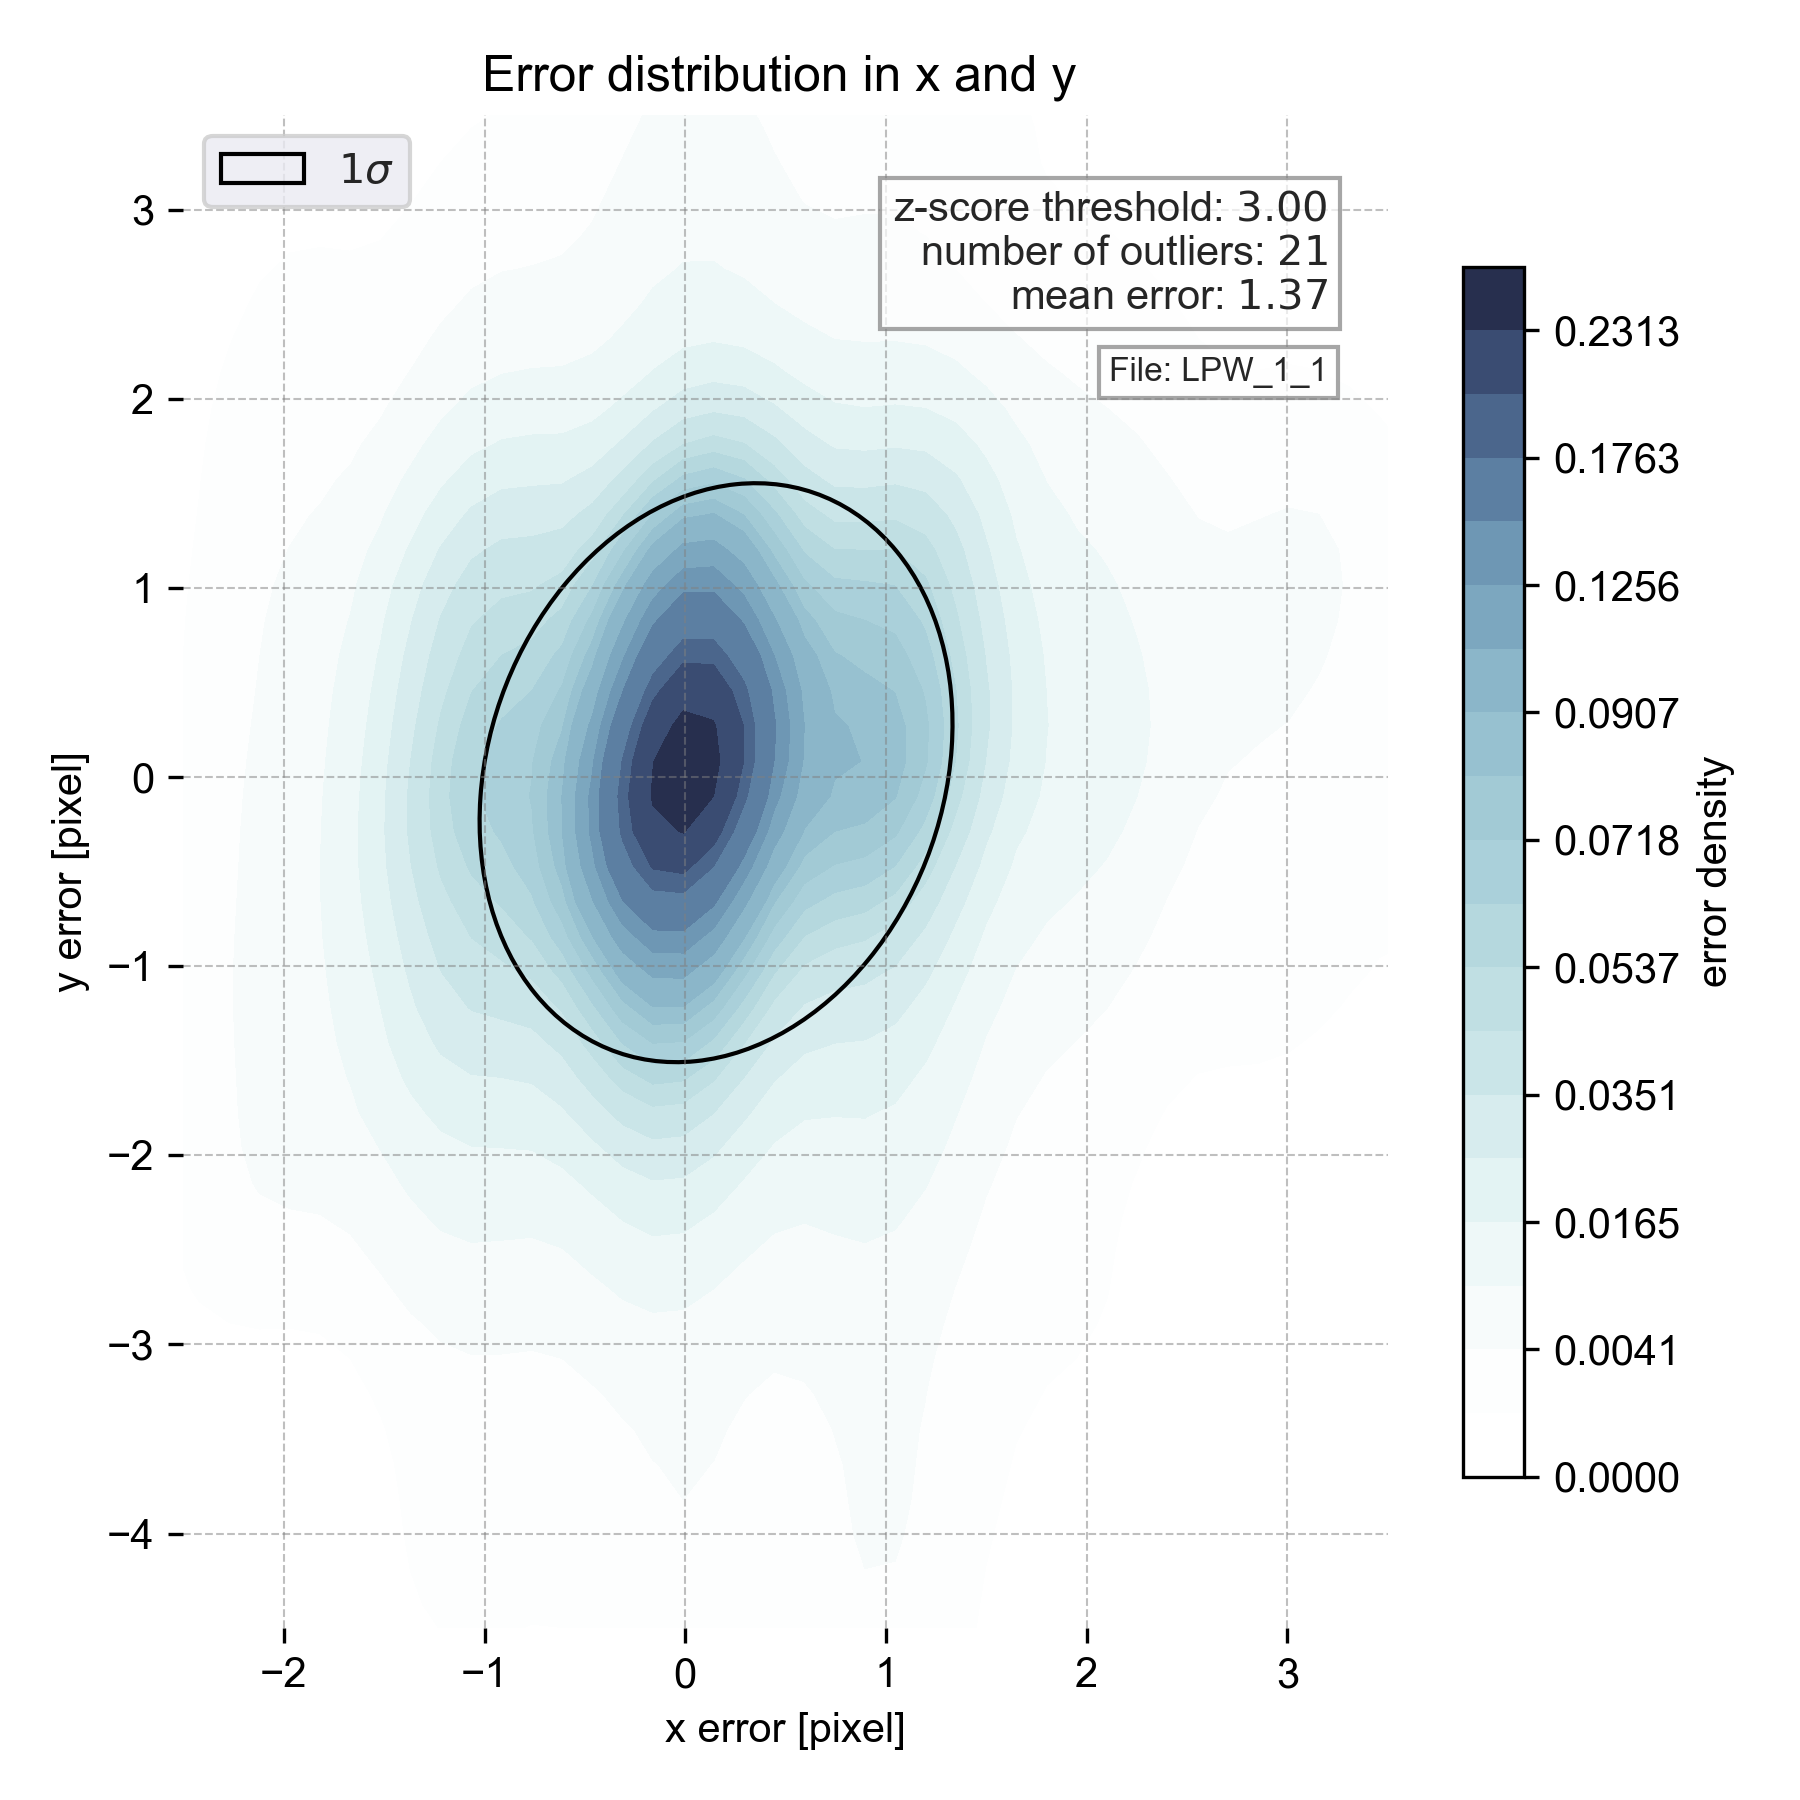
\includegraphics[width=\textwidth]{plots/LPW_1_1pre.png}
        \caption{Full image size (640x480)}
        \label{fig:full_scale}
    \end{subfigure}
    \begin{subfigure}{0.49\textwidth}
        \centering
        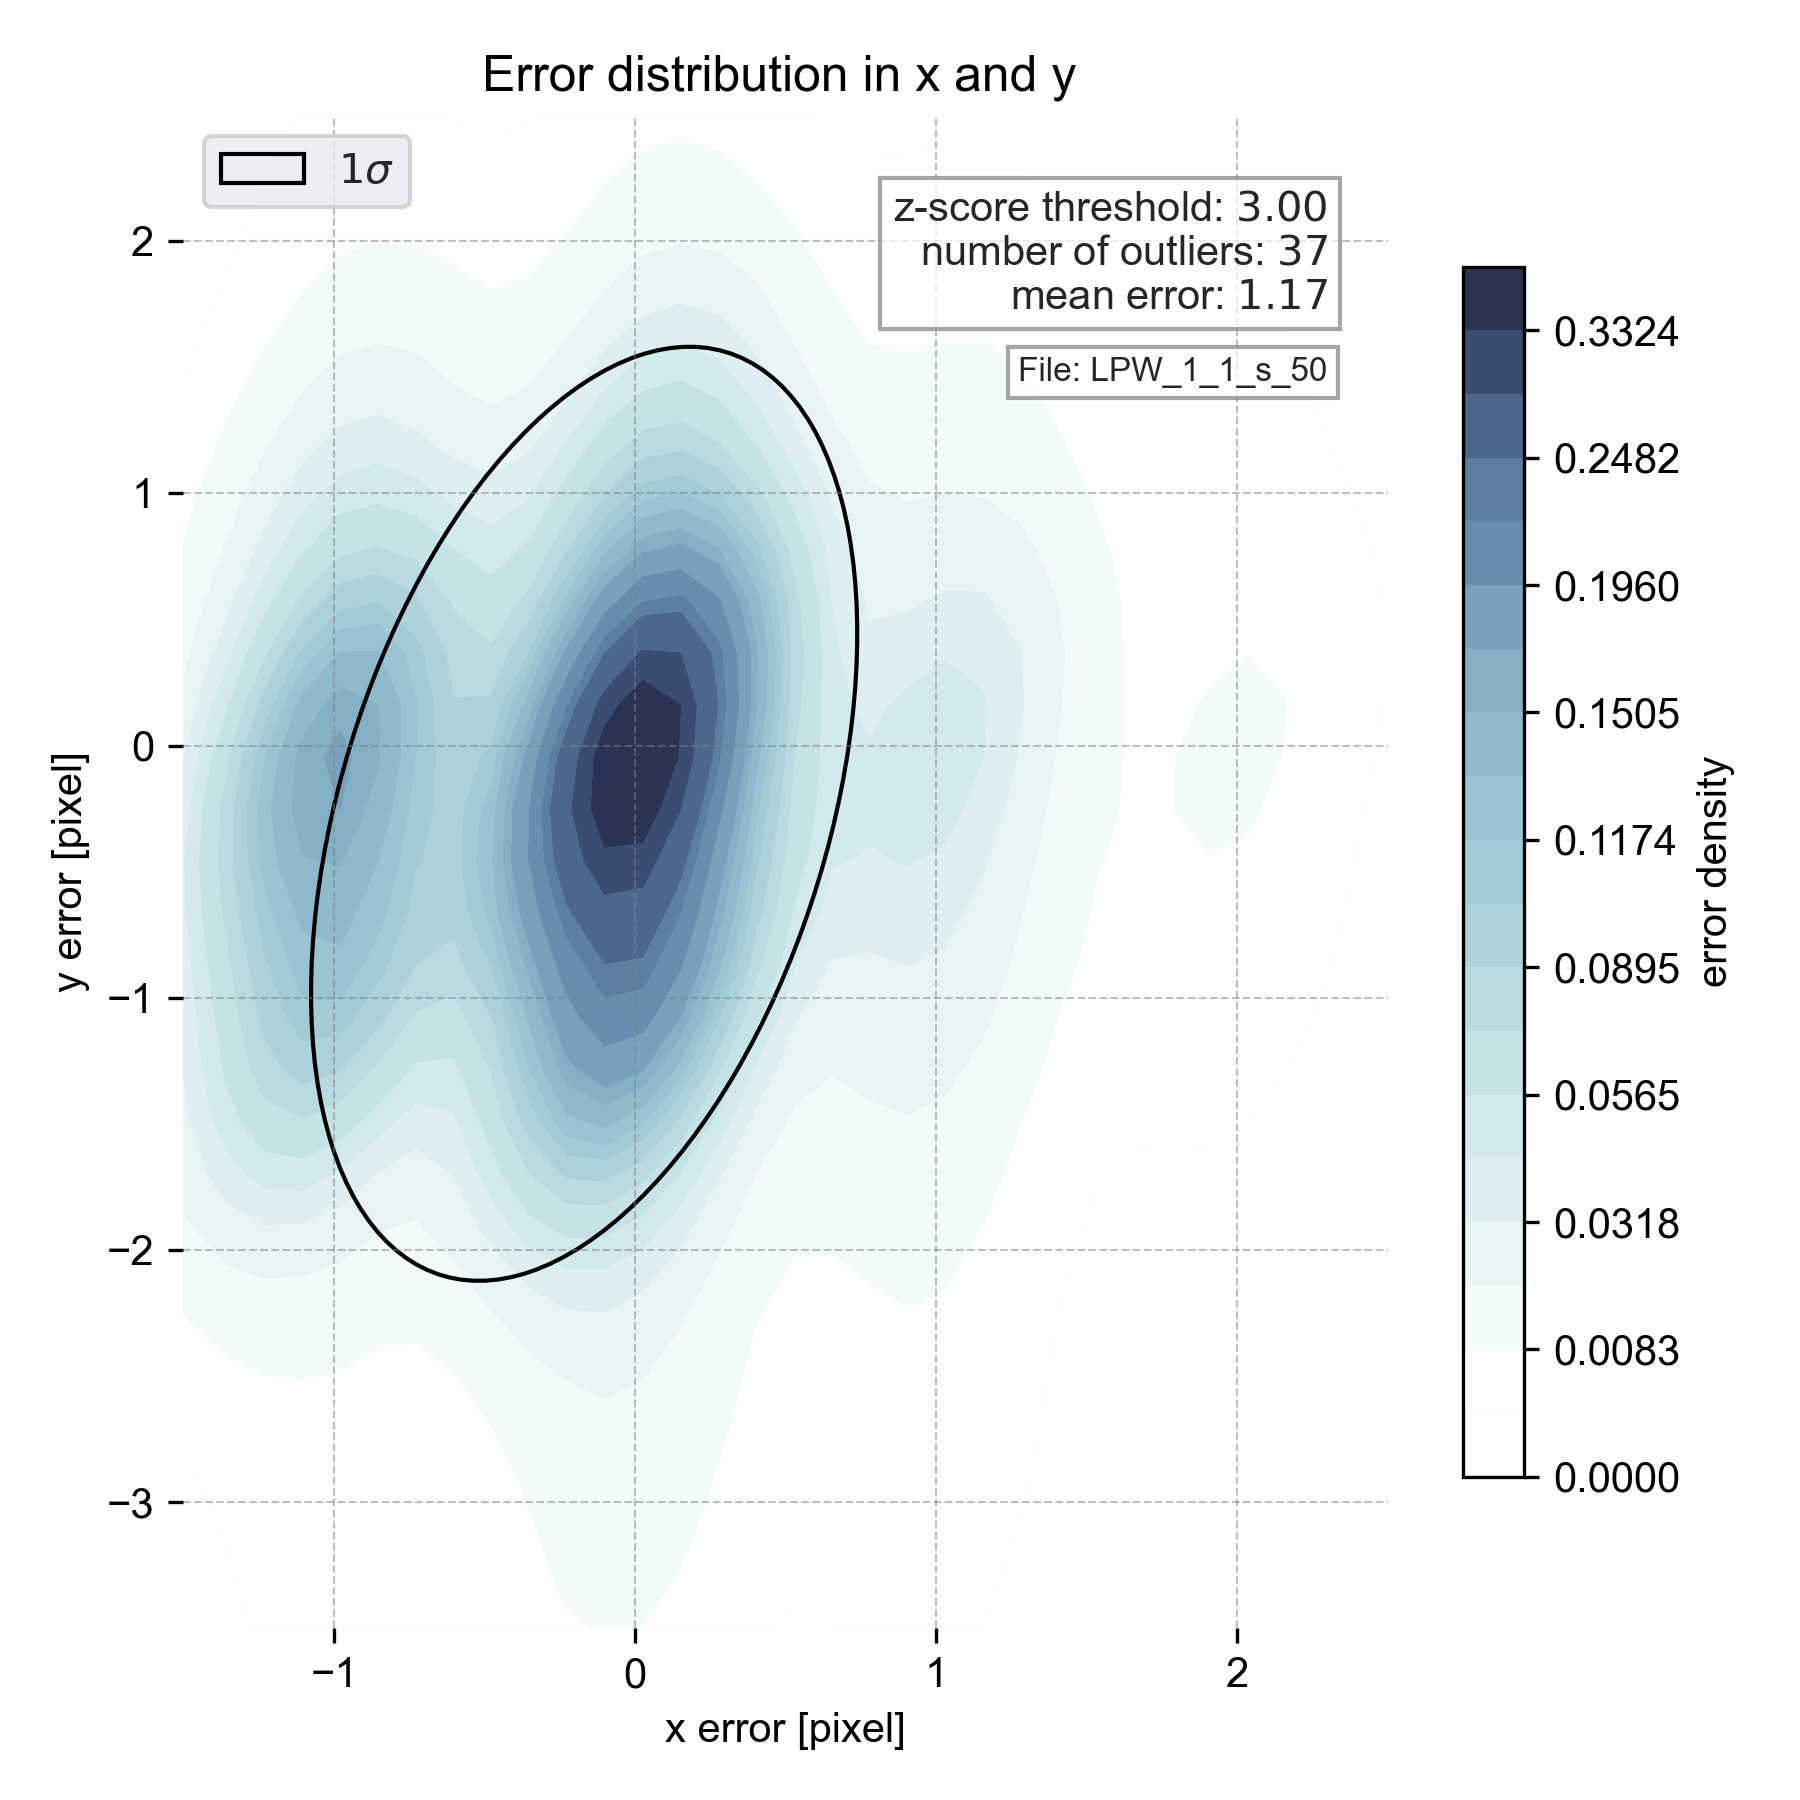
\includegraphics[width=\textwidth]{plots/LPW_1_1_s_50.png}
        \caption{Image size scaled by 0.5 (320x240)}
        \label{fig:halfscale}
    \end{subfigure}
    \caption{Comparing Error KDE plots of different image sizes}
    \label{fig:comp_e_size}
\end{figure}
Even thougth the mean error in figure \ref{fig:halfscale} seems to be lower, it needs to be considered that the number of outliers almost doubled when scaling the frames with a factor of 0.5 and the standard deviation also increases in the y direction. But notable is that the Haar-like feature was able to detect the pupil in every frame, no mather the scaling. This is not the case for all the videos in the LPW data set. By scaling the image information is lost including information about the pupil boundary. Important to note is that the parameters for the Haar-like feature and ACWE were adapted to the scaling of the images. 
It is possible to get more accurate results by increasing the number of iterations of the RANSAC algorithm aswell as $\lambda_1$ and $\lambda_2$ of the ACWE algorithm. This comes with the cost of speed, discussed in the next section. 
Another aspect of the accuracy is the fit of the ellipse itself. Even though the center has a considerable low error the fit of the ellipse also tends to be sort of jump in a range of one or two pixels. This effect can also be seen when using scaled frames but does not necessary increase with the scaling. The reason for this is the RANSAC algorithm that is used to fit the ellipse to the binary mask. This can be solved by using a higher number for iterations. The ACWE algorithm can also be a limiting factor because it stops at the outer boundary of the pupil which is not necessarily the same boundary as visually percepted.
\subsection{Speed}
The speed of the algorithm is measured by the time it takes to process 2000 frames. The mean of the total time per frame is considered the speed of the algorithm. Currently the algorithm runs at 1.3 fps, which equals 0.77 seconds per frame. This time was measured on full scale images of the size 640x480. Decreasing the size improves the duration significantly but also increases the mean error and decreases the success rate slightly. The parameters for the Haar-like feature and ACWE need to be recalibrated for the new scaling, there is not a general rule of thumb to scale the parameters. Also the the speed of the algorithm does not scale linearly with the size of the image.
\subsection{Robustness}
The robustness of the algorithm is measured by the amount of outliers the algorithm produces. By calculating the z-score and setting the threshold to three times the standard deviation of the complete video it is possible to filter outliers out and get a numerical value for the robustness. In a full scale image with reasonable noise, the haar like feature is able to find a point in the pupil in every frame. The smaller the image get, the less reliable the haar-like feature method becomes. But even at a scaling of 0.5 the Haar-like feature performs at a success rate of 99.5 percent. The ACWE algorithm is the limiting factor for the robustnes. Because the RANSAC algorithm expect a certain amount of boundary points to fit the ellipse to. If the ACWE algorithm is not able to extract the pupil area the error will be also visible in the boundary approximation. 
\subsection{Noise}

\section{Possible Improvements}
The algorithm has many parameters that can be tuned to imporve the performance. The parameters that can have a great impact on the performance are the parameters of the ACWE introduced in section \ref{sus:acwe_ransac} and RANSAC parametes introduced in section\ref{sus:ransac}. The parameters are:
\begin{gather*}
    \text{ACWE: } \lambda_1, \lambda_2,\text{smoothing iteratios}, \text{Iterations}\\
    \text{RANSAC: } \alpha, \beta, \text{Iterations}, \text{Threshold}
\end{gather*}
Because the binary mask of the ACWE is used for the RANSAC, $\lambda_1$ and $\lambda_2$ are of great importance for the accuracy of the model. If those parameters are chosen wrong, ACWE will not be able to extraxt the pupil area correctly and therefore the RANSAC will not be able to fit an accurate ellipse to the boundary of the pupil.

The number of Iterations is less of importance for the ACWE because it has a stopping criteria when the contour does not change anymore but has to be chosen high enough, so that the ACWE is not abruptly stoped before the contour has converged. If more smooting iterations are chosen, the contour will grow and converge faster but will also be more inaccurate. So there is a tradeoff between speed and accuracy. 

The RANSAC algorithm is also sensitive to the choice of parameters. $\alpha$ and $\beta$ do not have an influence on the speed but on the accuracy. They are the weights for the importance of inliers or boundary points. The number of iterations has an effect on the speed and accuracy. The more iterations are chosen, the more different ellipses are fitted and the chance for a better fit is higher with the cost of speed.

The $threshold$ that is used to decide if a point is on the boundary or not has also an effect on the accuracy. The reason why the threshold can have an impact on the accuracy is because the binary mask will not have a perfect elliptic boundary and therefore the RANSAC algorithm needs to have a certain threshold to decide if a point is on the boundary or not. 

To find the best values for the parameters more testing should be done. All in all, the proposed algorithm is currently not able to run at real time and still needs some improvements and bug fixing. To further improve the performance, the proposed algorithms should be implemented in C++ with more multithreading and parallelization. 

